% BANKS-SOURCE: pdf=167 print=157 kind=figure id=9.4
\tikzset{BanksNLoop/.style={line width=.55pt,dash pattern=on 3pt off 3pt},
         BanksNLeg/.style={line width=.55pt,dash pattern=on 3pt off 3pt}}
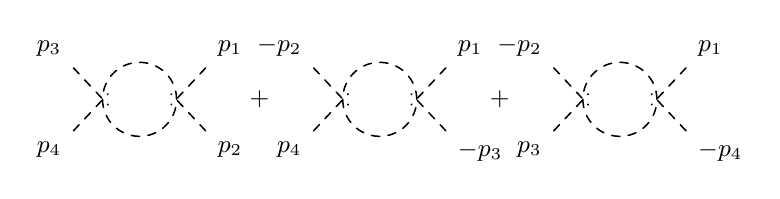
\begin{tikzpicture}[x=1cm,y=1cm,baseline=-.4ex,line cap=round,
  every node/.style={font=\small}]
  % Three one-loop bubbles.  At each vertex the two external legs cross,
  % overshooting slightly into the loop, exactly as in the source.
  \foreach \x in {0,3.05,6.10} {
    \draw[BanksNLoop] (\x,0) circle (.47);
    \draw[BanksNLeg] (\x-.84,.40) -- (\x-.40,-.07);
    \draw[BanksNLeg] (\x-.84,-.40) -- (\x-.40,.07);
    \draw[BanksNLeg] (\x+.84,.40) -- (\x+.40,-.07);
    \draw[BanksNLeg] (\x+.84,-.40) -- (\x+.40,.07);
  }
  \node at (1.525,0) {$+$};
  \node at (4.575,0) {$+$};
  % s-channel
  \node[anchor=south east] at (-.87,.42) {$p_3$};
  \node[anchor=north east] at (-.87,-.42) {$p_4$};
  \node[anchor=south west] at (.87,.42) {$p_1$};
  \node[anchor=north west] at (.87,-.42) {$p_2$};
  % t-channel
  \node[anchor=south east] at (2.18,.42) {$-p_2$};
  \node[anchor=north east] at (2.18,-.42) {$p_4$};
  \node[anchor=south west] at (3.92,.42) {$p_1$};
  \node[anchor=north west] at (3.92,-.42) {$-p_3$};
  % u-channel
  \node[anchor=south east] at (5.23,.42) {$-p_2$};
  \node[anchor=north east] at (5.23,-.42) {$p_3$};
  \node[anchor=south west] at (6.97,.42) {$p_1$};
  \node[anchor=north west] at (6.97,-.42) {$-p_4$};
\end{tikzpicture}
